\documentclass{article} % Tạo một bản báo cáo
\usepackage[utf8]{inputenc}
\usepackage[T5]{fontenc} % Để sử dụng Tiếng Việt
\usepackage[fontsize=13pt]{scrextend} % Set fontsize=13pt
\usepackage{forest}
\usepackage{diagbox} % for diagonal split box
\usepackage{array}
\usepackage[none]{hyphenat}
\usepackage[paperheight=29.7cm,paperwidth=21cm,right=2cm,left=3cm,top=2cm,bottom=2.5cm,twoside]{geometry}% Chuẩn A4, căn lề phải, trái, trên, dưới.
\usepackage{longtable}
\usepackage{newunicodechar}
\newunicodechar{Γ}{\ensuremath{\Gamma}}
\usepackage{mathptmx} % Time New Roman
\usepackage{amsmath}
\usepackage{graphicx} % Thư viện chèn ảnh
\usepackage{float} % Set vị trí chèn ảnh
\usepackage{tikz} % Thư viện tạo khung bìa
\usetikzlibrary{calc} % Thư viện tikz
\usepackage{indentfirst} % Thư viện thụt đầu dòng
\renewcommand{\baselinestretch}{1.2} % Giãn dòng 1.2
\setlength{\parskip}{6pt} % Spacing after
\setlength{\parindent}{1cm} % Set khoảng cách thụt đầu dòng mỗi đoạn
\usepackage{titlesec} % Thư viện để set up các kiểu chữ
\setcounter{secnumdepth}{4} % 4 Heading
\titlespacing*{\section}{0pt}{0pt}{30pt} % Heading 1
\titleformat*{\section}{\fontsize{16pt}{0pt}\selectfont \bfseries \centering}
\titlespacing*{\subsection}{0pt}{10pt}{0pt} % Heading 2
\titleformat*{\subsection}{\fontsize{14pt}{0pt}\selectfont \bfseries}
\titlespacing*{\subsubsection}{0pt}{10pt}{0pt} % Heading 3
\titleformat*{\subsubsection}{\fontsize{13pt}{0pt}\selectfont \bfseries \itshape}
\titlespacing*{\paragraph}{0pt}{10pt}{0pt} % Heading 4
\titleformat*{\paragraph}{\fontsize{13pt}{0pt}\selectfont \itshape}
\renewcommand{\figurename}{\fontsize{12pt}{0pt}\selectfont \bfseries Hình}
\renewcommand{\thefigure}{\thesection.\arabic{figure}}
\usepackage[font=bf]{caption}
\captionsetup[figure]{labelsep=space}
\renewcommand{\tablename}{\fontsize{12pt}{0pt}\selectfont \bfseries Bảng}
\renewcommand{\thetable}{\thesection.\arabic{table}}
\captionsetup[table]{labelsep=space}
\usepackage{tabularx}
\newcolumntype{s}{>{\hsize=.3\hsize}X}
\newcolumntype{y}{>{\hsize=.4\hsize}X}
\newcolumntype{d}{>{\hsize=.1\hsize}X}
\newcolumntype{a}{>{\hsize=1.1\hsize}X}
\newcolumntype{g}{>{\hsize=5\hsize}X}
\renewcommand{\tabularxcolumn}[1]{>{\raggedright\arraybackslash}p{#1}}

\renewcommand{\theequation}{\thesection.\arabic{equation}} % Thay đổi đánh số phương trình mặc định
\newtheorem{theorem}{Định lý}[section]
\newtheorem{defn}[theorem]{Định nghĩa}
\newtheorem{corollary}[theorem]{Hệ quả}
\newtheorem{lemma}[theorem]{Bổ đề}
\renewcommand{\contentsname}{MỤC LỤC}
\renewcommand{\listfigurename}{DANH MỤC HÌNH VẼ}
\renewcommand{\listtablename}{DANH MỤC BẢNG BIỂU}
\renewcommand{\refname}{TÀI LIỆU THAM KHẢO}
\usepackage[unicode]{hyperref}
\usepackage{colortbl}
\definecolor{LightCyan}{rgb}{0.88,1,1}
\begin{document}
\begin{titlepage}
\begin{tikzpicture}[overlay,remember picture]
\draw [line width=3pt]
    ($ (current page.north west) + (3.0cm,-2.0cm) $)
    rectangle
    ($ (current page.south east) + (-2.0cm,2.5cm) $);
\draw [line width=0.5pt]
    ($ (current page.north west) + (3.0cm,-2.1cm) $)
    rectangle
    ($ (current page.south east) + (-2.1cm,2.6cm) $); 
\end{tikzpicture}
\begin{center}
\vspace{-12pt}  ĐẠI HỌC BÁCH KHOA HÀ NỘI \\
\textbf{\fontsize{16pt}{0pt}\selectfont TRƯỜNG ĐIỆN - ĐIỆN TỬ}
\vspace{0.5cm}
 \begin{figure}[H]
     \centering
     \includegraphics[width=1.54cm,height=2.26cm]{images/logodhbk.png}
 \end{figure}
\vspace{1.5cm}
\textbf{\fontsize{32pt}{0pt}\selectfont ĐỒ ÁN ĐỀ XUẤT}
\vspace{1.5cm}
\end{center}
\hspace{6pt}\textbf{\fontsize{14pt}{0pt}\selectfont Đề tài:}
\begin{center}
    \textbf{\fontsize{18pt}{0pt}\selectfont NGHIÊN CỨU VỀ BÀI TOÁN SỬ DỤNG TRÍ TUỆ NHÂN TẠO ĐỂ TỐI ƯU CHO QUÁ TRÌNH CHUYỂN GIAO}\\

\vspace{1.5cm}
\begin{table}[H]
    \centering
    \begin{tabular}{l l}
 \fontsize{14pt}{0pt}\selectfont Học viên thực hiện:    & \fontsize{14pt}{0pt}\selectfont Dương Đình Nhật \vspace{6pt} \\ 
     &\fontsize{14pt}{0pt}\selectfont Kỹ thuật Điện tử (KH) - CH2024B \vspace{6pt}\\
\fontsize{14pt}{0pt}\selectfont Giảng viên hướng dẫn: & \fontsize{14pt}{0pt}\selectfont TS. Phùng Thị Kiều Hà
\end{tabular}
\end{table}
\vspace{3.5cm}
 \fontsize{14pt}{0pt}\selectfont Hà Nội, 20/09/2025
\end{center}
\end{titlepage}
 % Bìa đồ án.
 % Tạo mục lục tự động
\addtocontents{toc}{\protect\thispagestyle{empty}}
\tableofcontents
\thispagestyle{empty}
\cleardoublepage
\section*{DANH MỤC KÝ HIỆU VÀ CHỮ VIẾT TẮT}
\addcontentsline{toc}{section}{\numberline {} DANH MỤC KÝ HIỆU VÀ CHỮ VIẾT TẮT}
\begin{longtable}{|p{3.2cm}|p{11.3cm}|}
\hline
\textbf{Ký hiệu} & \textbf{Tên đầy đủ} \\
\hline
\endhead
3GPP & 3rd Generation Partnership Project \\
\hline
6G & Thế hệ mạng di động thứ 6 \\
\hline
NTN & Non-Terrestrial Network (mạng phi mặt đất) \\
\hline
LEO & Low Earth Orbit (quỹ đạo Trái Đất thấp) \\
\hline
MEO/\allowbreak GEO & Medium Earth Orbit / Geostationary Earth Orbit \\
\hline
UE & User Equipment (thiết bị người dùng) \\
\hline
HO & Handover (chuyển giao) \\
\hline
HOF & Handover Failure (chuyển giao thất bại) \\
\hline
RLF & Radio Link Failure (lỗi liên kết vô tuyến) \\
\hline
PP & Ping-Pong \\
\hline
BHO & Baseline Handover \\
\hline
CHO & Conditional Handover (chuyển giao có điều kiện) \\
\hline
DAPS & Dual Active Protocol Stack \\
\hline
RSRP/\allowbreak RSRQ & Reference Signal Received Power / Reference Signal Received Quality \\
\hline
SINR/\allowbreak SNR & Signal-to-Interference-plus-Noise Ratio / Signal-to-Noise Ratio \\
\hline
SE & Spectral Efficiency (hiệu suất phổ) \\
\hline
TTT & Time-to-Trigger \\
\hline
QoS/\allowbreak QoE & Quality of Service / Quality of Experience \\
\hline
JFI & Jain's Fairness Index \\
\hline
RVT & Remaining Visible Time \\
\hline
S-LEO/\allowbreak T-LEO & Source LEO satellite / Target LEO satellite \\
\hline
MR & Measurement Report \\
\hline
RIC/\allowbreak O-RAN & (near-)Real-time RAN Intelligent Controller / Open RAN \\
\hline
FCC & Federal Communications Commission \\
\hline
VSAT & Very Small Aperture Terminal \\
\hline
GAP & Generalized Assignment Problem \\
\hline
ML/\allowbreak AI & Machine Learning / Artificial Intelligence \\
\hline
RL/\allowbreak DRL & (Deep) Reinforcement Learning \\
\hline
MARL & Multi-Agent Reinforcement Learning \\
\hline
MDP & Markov Decision Process \\
\hline
DQN & Deep Q-Network \\
\hline
IQL & Independent Q-Learning \\
\hline
VDN & Value-Decomposition Networks \\
\hline
QMIX & Tên thuật toán MARL dùng trong bài báo gốc (không phải chữ viết tắt) \\
\hline
CTDE & Centralized Training, Decentralized Execution \\
\hline
DRQN & Deep Recurrent Q-Network \\
\hline
GRU & Gated Recurrent Unit \\
\hline
PPO/\allowbreak MADDPG/\allowbreak MAPPO & Tên các thuật toán DRL/MARL khác \\
\hline
ILCHO & Intelligent LEO satellite Conditional Handover \\
\hline
MD-CHO/\allowbreak MVT-CHO & Minimum-Distance CHO / Maximum-Visible-Time CHO \\
\hline
HSNF/\allowbreak LBSH & Tên hai phương pháp so sánh (baseline) trong bài báo gốc \\
\hline
TLE & Two-Line Element \\
\hline
\end{longtable}
 % Danh mục ký hiệu và chữ viết tắt
%Tạo danh mục hình vẽ.
{\let\oldnumberline\numberline
\renewcommand{\numberline}{Hình~\oldnumberline}
\listoffigures}
\newpage
\phantomsection\addcontentsline{toc}{section}{\numberline {} DANH MỤC HÌNH VẼ}
\newpage
 %Tạo danh mục bảng biểu.
{\let\oldnumberline\numberline
\renewcommand{\numberline}{Bảng~\oldnumberline}
\listoftables}
\phantomsection\addcontentsline{toc}{section}{\numberline {} DANH MỤC BẢNG BIỂU}
\newpage
\section*{TÓM TẮT ĐỒ ÁN}
\addcontentsline{toc}{section}{\numberline {}TÓM TẮT ĐỒ ÁN}
6G hướng tới phủ sóng toàn cầu bằng mạng phi mặt đất (NTN), trong đó vệ tinh quỹ đạo thấp (LEO) là thành phần then chốt. Do bay nhanh và vùng phủ hẹp, một thiết bị người dùng (UE) trong chòm vệ tinh LEO mật độ cao (kiểu Starlink) phải chuyển giao (handover) liên tục, trong khi việc đo tín hiệu kiểu mạng mặt đất không còn đáng tin cậy. Bài báo \textit{``Intelligent Handover Scheme for Improved 6G NTN LEO Satellite Network Performance''} (gọi tắt \textbf{ILCHO}) đề xuất kết hợp cơ chế Chuyển giao có điều kiện (Conditional Handover - CHO) của 3GPP với học tăng cường đa tác tử (QMIX) để chọn vệ tinh đích cho từng UE, dựa trên nền tảng giải tích chứng minh vị trí vệ tinh là tất định và bài toán gán tối ưu là NP-hard.

Trong đồ án này, em thực hiện hai phần việc chính. \textbf{Thứ nhất}, em khảo sát (survey) và phân tích chi tiết bài báo ILCHO: bối cảnh, mô hình hệ thống, thiết kế thuật toán, kết quả công bố, đồng thời chỉ ra các điểm mạnh, hạn chế và khoảng trống nghiên cứu khi đặt bài báo vào bức tranh chung của các phương pháp AI cho handover. \textbf{Thứ hai}, vì bài báo không công khai mã nguồn và không công bố đầy đủ tham số, em tự xây dựng lại toàn bộ mô hình (hình học chòm vệ tinh, mô hình kênh 3GPP, môi trường mô phỏng CHO đa tác tử, bộ điều khiển QMIX và bốn phương pháp so sánh) để tái hiện thực nghiệm, huấn luyện qua ba lượt tăng dần quy mô tới đúng quy mô bài báo công bố (100 UE, 600 giây/lượt phục vụ), và kiểm chứng độ ổn định qua nhiều lần huấn luyện độc lập (seed).

Kết quả tái hiện cho thấy tuyên bố cốt lõi của bài báo — cơ chế CHO điều khiển bằng học tăng cường đa tác tử giữ số chuyển giao thất bại thấp và ổn định trong chòm vệ tinh mật độ cao, trong khi các phương pháp truyền thống (chọn vệ tinh gần nhất, chọn vệ tinh có thời gian nhìn thấy lâu nhất) sụp đổ khi tải tăng — được tái hiện rõ ràng và vững chắc, đặc biệt khi huấn luyện đúng quy mô bài báo. Đồng thời, em cũng phát hiện và báo cáo trung thực hai điểm không tái hiện được (thông lượng cao nhất; sự bất ổn của biến thể hàm thưởng tuyến tính), cùng các hạn chế còn tồn tại do một số tham số quan trọng không được bài báo công bố.

\vspace{6pt}
\noindent\textbf{Từ khóa:} 6G, mạng phi mặt đất (NTN), vệ tinh LEO, chuyển giao có điều kiện (CHO), học tăng cường đa tác tử (MARL), QMIX, ILCHO.
 % Tóm tắt đồ án
\pagenumbering{arabic} % Đánh số thứ tự 1,2,3...

\section*{CHƯƠNG 1. ĐẶT VẤN ĐỀ}
\addcontentsline{toc}{section}{\numberline{}CHƯƠNG 1. ĐẶT VẤN ĐỀ}
\setcounter{section}{1}
\setcounter{subsection}{0}
\setcounter{figure}{0}
\setcounter{table}{0}

\subsection{Bối cảnh: 6G và mạng phi mặt đất (NTN) dùng vệ tinh LEO}
Bên cạnh việc tăng tốc độ dữ liệu, một trong những mục tiêu quan trọng nhất của 6G là \textbf{phủ sóng toàn cầu}, kể cả những nơi mạng mặt đất (Terrestrial Network - TN) không thể vươn tới hoặc dễ sập khi có thiên tai: vùng nông thôn, biển đảo, hành khách trên máy bay/tàu biển, hay các ứng dụng IoT mật độ cao ở vùng thưa dân. Mạng phi mặt đất (Non-Terrestrial Network - NTN) — dùng vệ tinh, khinh khí cầu tầng cao (HAPS) hay máy bay không người lái — được 3GPP đưa vào lộ trình chuẩn hoá từ Release 15 để giải quyết đúng bài toán này.

Trong các tầng quỹ đạo vệ tinh, \textbf{vệ tinh quỹ đạo thấp (Low Earth Orbit - LEO, cao độ 300--2.000 km)} được xem là mảnh ghép quan trọng nhất cho 6G vì có độ trễ truyền thấp nhất (tối đa khoảng 12,89 ms, so với 270,73 ms của vệ tinh địa tĩnh - GEO) và suy hao đường truyền nhỏ hơn. Đánh đổi là \textbf{vùng phủ sóng của một vệ tinh LEO rất hẹp và thời gian phủ một điểm trên mặt đất rất ngắn} (do vệ tinh bay rất nhanh, khoảng 7,6 km/s ở độ cao 550 km), nên để phủ sóng liên tục, các nhà mạng phải triển khai \textbf{chòm vệ tinh mật độ rất cao} — điển hình là Starlink, theo hồ sơ của Ủy ban Truyền thông Liên bang Hoa Kỳ (FCC) đã quy hoạch tới gần 30.000 vệ tinh ở Phase 2 và tính đến đầu 2025 đã có khoảng 8.000 vệ tinh được phóng.

\subsection{Bài toán chuyển giao trong mạng vệ tinh LEO mật độ cao}
Hệ quả trực tiếp của việc vùng phủ mỗi vệ tinh hẹp và vệ tinh di chuyển liên tục là một thiết bị người dùng (User Equipment - UE), kể cả khi đứng yên trên mặt đất, cũng phải thực hiện \textbf{chuyển giao (handover - HO)} sang vệ tinh khác một cách thường xuyên. Theo 3GPP TR 38.821 \cite{3gpp38821}, chu kỳ chuyển giao của LEO rơi vào khoảng \textbf{6,61 -- 132,28 giây} tùy vị trí UE so với vùng phủ. Đây là tần suất chuyển giao cao hơn rất nhiều so với mạng mặt đất, khiến quản lý di động trở thành một nút thắt hiệu năng thực sự của NTN.

Khó khăn còn nằm ở việc \textbf{đo tín hiệu kiểu mạng mặt đất không còn đáng tin cậy}: các "cell" vệ tinh ở rất xa (hàng trăm km), tín hiệu từ nhiều vệ tinh chồng lấn và dao động khó lường, nên UE khó phân biệt được vệ tinh nào thực sự tốt hơn chỉ dựa vào đo công suất tín hiệu tham chiếu (RSRP) như ở 5G mặt đất. Cơ chế chuyển giao truyền thống (Baseline Handover - BHO) — quyết định \emph{phản ứng (reactive)}, chỉ chuẩn bị chuyển giao khi tín hiệu đã suy giảm — dễ dẫn tới \textbf{lỗi liên kết vô tuyến (RLF)} và \textbf{chuyển giao thất bại (HOF)} trong môi trường LEO tốc độ cao. 3GPP kết luận không nên áp dụng nguyên xi thuật toán HO của TN vào NTN, và đề xuất \textbf{Chuyển giao có điều kiện (Conditional Handover - CHO, Release 16)}: mạng chuẩn bị trước một số vệ tinh ứng viên, UE tự chủ động chuyển giao khi một điều kiện định trước được thoả (theo phép đo, vị trí, timing-advance hoặc góc ngẩng), thay vì luôn phải chờ đo đạc và báo cáo về mạng.

Tuy nhiên, CHO của 3GPP mới chỉ giải quyết \textbf{cách thức} chuyển giao chủ động, chứ \textbf{chưa trả lời câu hỏi cốt lõi: khi có hàng chục đến hàng trăm UE cùng tồn tại và cạnh tranh tài nguyên, nên chọn vệ tinh đích nào là tốt nhất cho từng UE?} Nếu chỉ dùng các tiêu chí đơn giản (khoảng cách gần nhất, thời gian nhìn thấy lâu nhất), nhiều UE ở gần nhau có xu hướng cùng chọn một vệ tinh "tốt nhất" theo cùng tiêu chí, gây nghẽn tài nguyên và số lần chuyển giao thất bại tăng vọt khi tải hệ thống tăng — một hạn chế lớn của cả phương pháp truyền thống lẫn nhiều công trình học máy công bố trước đây khi mở rộng lên quy mô một chòm vệ tinh thương mại thực thụ như Starlink.

\subsection{Vai trò của học tăng cường đa tác tử và mục tiêu đồ án}
Bài toán chọn vệ tinh đích cho nhiều UE cùng lúc, dưới ràng buộc tài nguyên hữu hạn và mục tiêu vừa tối đa hiệu năng hệ thống vừa hạn chế số lần chuyển giao, về bản chất là một bài toán \textbf{ra quyết định tuần tự, nhiều tác tử, có ràng buộc} — rất phù hợp để giải bằng \textbf{Học tăng cường đa tác tử (Multi-Agent Reinforcement Learning - MARL)}. Đây chính là hướng tiếp cận được đề xuất trong bài báo \textit{"Intelligent Handover Scheme for Improved 6G NTN LEO Satellite Network Performance"} \cite{choi2026ilcho} — gọi tắt là \textbf{ILCHO} — kết hợp CHO của 3GPP với thuật toán MARL QMIX để chọn vệ tinh đích, đồng thời chứng minh bằng giải tích rằng bài toán gán tối ưu chính xác là NP-hard nên cần một phương pháp học xấp xỉ có khả năng mở rộng.


\newpage
\section*{CHƯƠNG 2. TỔNG QUAN BÀI BÁO ILCHO}
\addcontentsline{toc}{section}{\numberline{}CHƯƠNG 2. TỔNG QUAN BÀI BÁO ILCHO}
\setcounter{section}{2}
\setcounter{subsection}{0}
\setcounter{figure}{0}
\setcounter{table}{0}

\subsection{Tổng quan}
Tổng quan bao gồm 4 yếu tố chính:
\begin{enumerate}
    \item \textbf{Nền tảng giải tích} gồm ba Lemma: chứng minh vị trí vệ tinh là hàm \emph{tất định} theo thời gian, suy ra điều kiện "khả kiến" (accessible) của mỗi UE với từng vệ tinh mà không cần đo đạc thời gian thực, và chứng minh bài toán gán tối ưu là \textbf{NP-hard}.
    \item \textbf{Môi trường mô phỏng thực tế}: dùng tham số Starlink thật lấy từ hồ sơ FCC (Phase 1-a $\approx$550 km, Phase 2-a $\approx$340 km và kịch bản hybrid), thay vì mô hình giả định dưới 100 vệ tinh như phần lớn công trình trước.
    \item \textbf{Công thức MARL khả mở rộng}: không gian hành động của mỗi agent chỉ bằng số vệ tinh \emph{khả kiến tối đa} $N_{\max}$ (suy từ Lemma 2), không phải tổng số vệ tinh toàn hệ thống — nhờ đó độ phức tạp huấn luyện và suy luận \textbf{tuyến tính theo số UE}, không phụ thuộc tổng số vệ tinh. Đây là điểm kỹ thuật giá trị nhất của bài báo.
    \item \textbf{Kiểm chứng thực nghiệm}: theo nhóm tác giả, đây là nghiên cứu đầu tiên kiểm chứng CHO điều khiển bằng RL trên một mega-constellation LEO thương mại thực thụ.
\end{enumerate}

\subsection{Mô hình hệ thống và ba Lemma nền tảng}
Chòm vệ tinh được mô hình hoá theo cấu hình \textbf{Walker-Delta}: $M$ vệ tinh chia đều trên $N_p$ mặt phẳng quỹ đạo cùng góc nghiêng, mỗi mặt phẳng cách đều nhau về góc lên thiên đỉnh (RAAN), các vệ tinh trong một mặt phẳng cách đều pha.

\textbf{Lemma 1 (trạng thái vị trí vệ tinh).} Toạ độ Descartes của một vệ tinh tại thời điểm $t$ là một hàm tường minh của các tham số quỹ đạo (góc nghiêng, RAAN, pha ban đầu) và thời gian, suy ra trực tiếp từ định luật Kepler. Ý nghĩa cốt lõi: \textbf{vị trí vệ tinh tính trước được hoàn toàn từ tham số quỹ đạo (ephemeris), không cần đo đạc thời gian thực} — đây là nền tảng để ILCHO "biết trước" trạng thái vệ tinh thay vì phải đo tín hiệu như cách làm truyền thống.

\textbf{Lemma 2 (điều kiện khả kiến).} Từ Lemma 1 và vị trí (cố định) của UE, bài báo suy ra một điều kiện đại số cho biết UE có "nhìn thấy" một vệ tinh với góc ngẩng đủ lớn hay không, tại bất kỳ thời điểm nào, mà không cần quét từng cặp UE--vệ tinh theo thời gian thực. Nhờ đó, \textbf{tập vệ tinh khả kiến của mỗi UE, và số lượng vệ tinh khả kiến tối đa $N_{\max}$, tính trước được toàn bộ} — con số $N_{\max}$ này sau đó được dùng làm kích thước không gian hành động của MARL. Hình \ref{fig:accessible} minh hoạ số vệ tinh khả kiến trung bình thay đổi theo vĩ độ trạm mặt đất, tính từ chính mô hình hình học mà em dựng lại theo Lemma 2 — giá trị đỉnh của đường cong này chính là $N_{\max}$ dùng làm kích thước không gian hành động.

\begin{figure}[H]
\centering
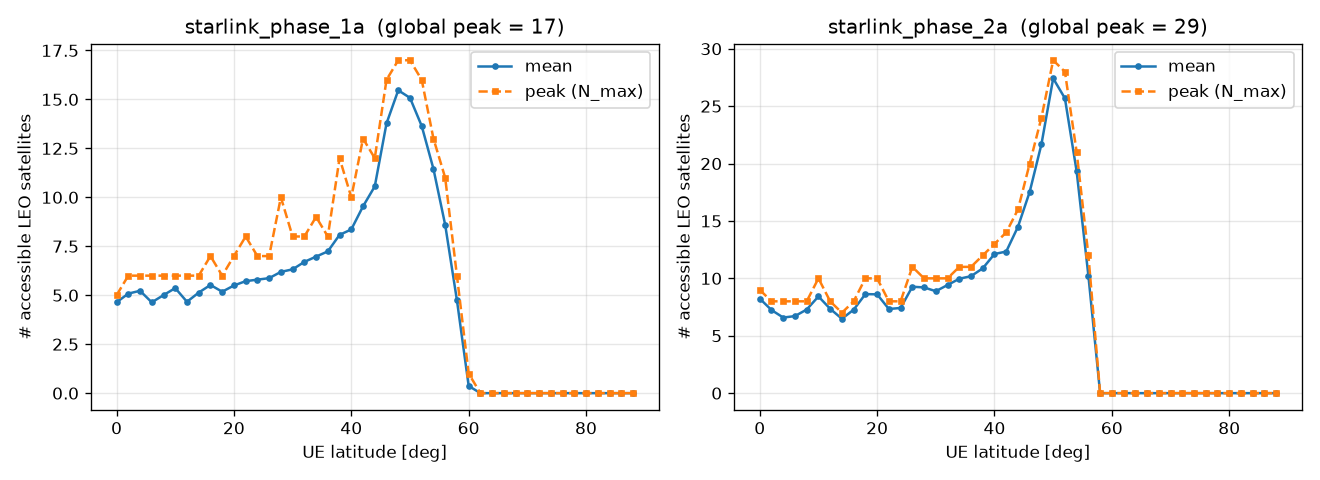
\includegraphics[width=0.8\textwidth]{images/analysis_fig5_accessible_vs_latitude.png}
\caption{Số vệ tinh khả kiến trung bình theo vĩ độ trạm mặt đất (minh hoạ Lemma 2).}
\label{fig:accessible}
\end{figure}

\textbf{Lemma 3 (độ phức tạp bài toán).} Với mô hình kênh 3GPP TR 38.811/38.821 \cite{3gpp38811,3gpp38821} để tính công suất thu và thông lượng Shannon, bài toán tối ưu "chọn UE nào kết nối vệ tinh nào để tối đa tổng thông lượng, với ràng buộc mỗi UE tối đa một vệ tinh và mỗi vệ tinh tối đa $J$ kênh" được quy về một \textbf{bài toán gán tổng quát (Generalized Assignment Problem - GAP)} tại mỗi lát thời gian, vốn là bài toán \textbf{NP-hard} kinh điển — do đó bài toán động (trên toàn bộ thời gian phục vụ) cũng NP-hard. Đây là căn cứ để nhóm tác giả chuyển sang dùng học máy (MARL) tìm lời giải xấp xỉ thay vì giải chính xác. Hình \ref{fig:linkbudget} minh hoạ quan hệ giữa công suất/SNR thu được và góc ngẩng của vệ tinh theo mô hình kênh này — góc ngẩng càng lớn (vệ tinh càng gần thiên đỉnh) thì suy hao đường truyền càng nhỏ, SNR và thông lượng Shannon càng cao, đúng như cơ sở để bài báo thiết kế hàm thưởng dạng sigmoid ở Mục 2.4.

\begin{figure}[H]
\centering
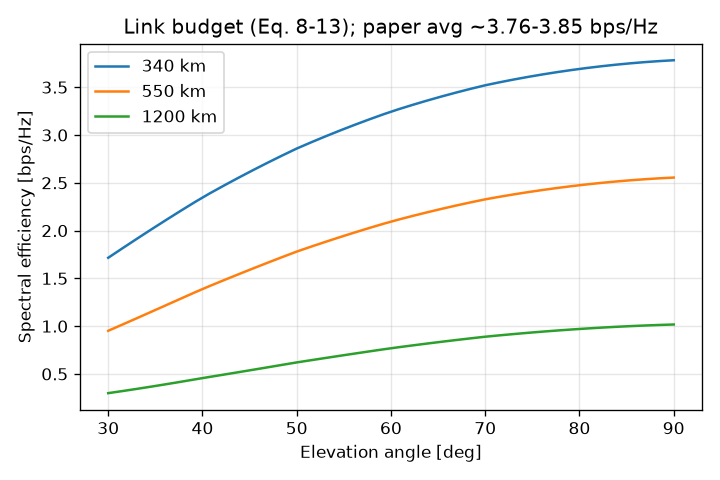
\includegraphics[width=0.8\textwidth]{images/analysis_link_budget_vs_elevation.png}
\caption{Công suất thu/SNR theo góc ngẩng của vệ tinh, tính theo mô hình kênh 3GPP TR 38.811/38.821.}
\label{fig:linkbudget}
\end{figure}

\subsection{Quy trình CHO ba pha và bộ điều khiển QMIX}
ILCHO chỉ can thiệp vào \textbf{pha chuẩn bị} của quy trình CHO ba pha theo 3GPP TS 38.300 \cite{3gpp38300}:
\begin{itemize}
    \item \textbf{Chuẩn bị (Preparation)}: khi sự kiện chuẩn bị thoả, UE gửi báo cáo đo (MR) tới vệ tinh nguồn (S-LEO). \textbf{Vệ tinh đích tối ưu (T-LEO) được chọn bằng thuật toán MARL} dựa trên ephemeris và trạng thái hiện tại; S-LEO cấu hình các T-LEO ứng viên và giữ trước tài nguyên vô tuyến cho UE (thời hạn hiệu lực của dữ liệu ephemeris dùng cho quyết định này được quản lý qua bộ định thời T430 theo 3GPP TS 38.331 \cite{3gpp38331}).
    \item \textbf{Thực thi (Execution)}: khi một sự kiện dựa trên \emph{khoảng cách} (biến thể của sự kiện A3 truyền thống, dùng khoảng cách thay vì RSRP) được thoả, UE thực sự chuyển sang T-LEO.
    \item \textbf{Hoàn tất (Completion)}: giống chuyển giao truyền thống — mạng lõi cập nhật đường truyền dữ liệu.
\end{itemize}
Nói cách khác, phần "trí tuệ" của ILCHO chỉ nằm ở việc \textbf{chọn vệ tinh đích nào} (pha chuẩn bị), còn \textbf{thời điểm} chuyển giao vẫn dùng một luật cố định dựa trên khoảng cách.

Nền tảng của bộ điều khiển là học tăng cường (Q-learning và mạng Q sâu - DQN) \cite{sutton2018rl,mnih2015dqn}, mở rộng lên nhiều tác tử. Để chọn T-LEO, bài báo dùng \textbf{QMIX} \cite{rashid2018qmix} — một thuật toán MARL dựa trên giá trị (value-based), được chọn thay vì MADDPG (kém trong bài toán hợp tác, khó mở rộng) hay MAPPO (mạnh nhưng hội tụ chậm hơn trong bài toán này). Mỗi UE là một agent với thông tin cục bộ không đầy đủ; huấn luyện theo nguyên tắc \textbf{CTDE (Centralized Training, Decentralized Execution)}: dùng thông tin toàn cục lúc huấn luyện, nhưng khi thực thi mỗi agent chỉ cần quan sát cục bộ của chính nó. Mỗi agent có một mạng nơ-ron hồi quy (DRQN, dùng GRU để nhớ lịch sử quan sát) để ước lượng giá trị hành động cục bộ $Q_k$; một \emph{mixing network} (với trọng số không âm sinh ra bởi một hypernetwork) trộn các $Q_k$ thành giá trị toàn cục $Q_{tot}$ theo ràng buộc \textbf{đơn điệu}: hành động tham lam cục bộ của từng agent luôn làm tăng $Q_{tot}$. Đây chính là cách QMIX khắc phục vấn đề \emph{non-stationarity} (môi trường "không đứng yên" dưới góc nhìn một agent vì các agent khác cũng đang học) — nhược điểm cố hữu của các phương pháp học độc lập như IQL (Independent Q-Learning) \cite{sunehag2017vdn} mà nhiều công trình MARL trước đó sử dụng.

\subsection{Thiết kế bài toán MARL của ILCHO}
Mỗi UE $k$ là một agent quan sát cục bộ tại bước thời gian $t$:
\begin{itemize}
    \item \textbf{Trạng thái/quan sát}: danh sách $N_{\max}$ vệ tinh khả kiến, mỗi vệ tinh gồm 4 đặc trưng — chỉ số logic, khoảng cách tới UE, số kênh đang được sử dụng, và \textbf{thời gian còn khả kiến (Remaining Visible Time - RVT)}.
    \item \textbf{Hành động}: chọn 1 trong $N_{\max}$ vệ tinh khả kiến làm vệ tinh đích (T-LEO).
    \item \textbf{Hàm thưởng}: phạt nặng khi chuyển giao thất bại (HOF), phạt nhẹ hơn khi chuyển giao thành công (để hạn chế chuyển giao không cần thiết), và trong các bước còn lại dùng một \textbf{hàm chi phí dạng sigmoid} kết hợp thông lượng và RVT. Lý do dùng sigmoid thay vì hàm tuyến tính: thông lượng của một vệ tinh biến thiên \emph{không đơn điệu} theo thời gian (tăng khi vệ tinh tiến gần thiên đỉnh rồi giảm khi ra xa) trong khi RVT giảm đơn điệu, nên một hàm tuyến tính đơn giản dễ định giá sai các vệ tinh ở hai đầu; hàm sigmoid tạo ra một "điểm ngọt" tránh được vấn đề này. Bài báo có hẳn một thí nghiệm đối chứng (huấn luyện với hàm thưởng tuyến tính) để minh hoạ lập luận này. Đáng chú ý, hàm thưởng \textbf{không có số hạng cân bằng tải tường minh}, nhưng vì HOF hay xảy ra ở các vệ tinh quá tải nên việc phạt nặng HOF khiến agent \emph{tự học} cách né các vệ tinh đông đúc.
\end{itemize}
Toàn bộ quy trình huấn luyện (Algorithm 1 trong bài báo) được thực hiện tại một bộ điều khiển tập trung dạng \textbf{near-real-time RIC} theo kiến trúc O-RAN, còn vệ tinh chỉ cần chạy suy luận (inference) khi vận hành thực tế. Nhờ thiết kế không gian hành động $=N_{\max}$ (hằng số, không phụ thuộc tổng số vệ tinh), độ phức tạp huấn luyện và suy luận của ILCHO là \textbf{$O(K)$ — tuyến tính theo số UE $K$}, không phụ thuộc tổng số vệ tinh trong chòm sao.

\subsection{Công trình liên quan và bốn phương pháp so sánh}
Bài báo phân loại các công trình liên quan theo hướng tiếp cận (Bảng \ref{tab:related}) và chọn ra bốn phương pháp so sánh (baseline), đại diện cho hai nhóm — heuristic đơn tiêu chí và MARL không cắt gọn không gian hành động — để chỉ ra cả hai đều "sụp" khi số UE tăng.

\begin{table}[h!]
\centering
\caption{Các hướng tiếp cận liên quan và hạn chế được bài báo ILCHO chỉ ra.}
\label{tab:related}
\begin{tabular}{|>{\raggedright\arraybackslash}p{3.2cm}|>{\raggedright\arraybackslash}p{4.8cm}|>{\raggedright\arraybackslash}p{5cm}|}
\hline
\textbf{Hướng tiếp cận} & \textbf{Ý tưởng} & \textbf{Hạn chế (theo ILCHO)} \\
\hline
Lý thuyết trò chơi & Tối đa lợi ích UE bằng potential game & Không học, giả định lý tưởng \\
\hline
Network-flow (HSNF) & Đồ thị luồng, chi phí = thông lượng + băng thông còn lại & Tính chi phí mọi cặp UE--vệ tinh theo thời gian thực bất khả thi ở quy mô mega-constellation \\
\hline
RL đa tác tử độc lập (LBSH) & Q-learning độc lập, thưởng = RVT + tải + phạt HO & Không gian hành động nổ khi ghép vào Starlink, khó hội tụ \\
\hline
DQN + OneWeb & Tối đa thông lượng & Bỏ qua chi phí báo hiệu do HO thừa \\
\hline
DRL vệ tinh tự quyết & Vệ tinh nguồn tự chọn, UE không gửi báo cáo đo & Chỉ xét 3 mặt phẳng quỹ đạo $\Rightarrow$ "lời nguyền số chiều" khi lên chòm sao thật \\
\hline
\end{tabular}
\end{table}

\textbf{Bốn baseline dùng để so sánh với ILCHO:}
\begin{itemize}
    \item \textbf{MD-CHO} (Minimum Distance): chọn vệ tinh khả kiến gần nhất.
    \item \textbf{MVT-CHO} (Maximum Visible Time): chọn vệ tinh có RVT dài nhất.
    \item \textbf{HSNF}: gán tham lam tối đa hoá thông lượng tức thời có ràng buộc dung lượng (network-flow).
    \item \textbf{LBSH}: học tăng cường đa tác tử độc lập kết hợp thưởng cân bằng tải.
\end{itemize}
Thông điệp so sánh của bài báo: heuristic đơn tiêu chí (MD/MVT) sụp vì nhiều UE ở gần nhau cùng chọn một vệ tinh "tốt nhất" theo cùng tiêu chí $\Rightarrow$ nghẽn; LBSH sụp vì không gian hành động không được cắt gọn khi lên quy mô Starlink; ILCHO ổn định nhờ cả ba yếu tố: hàm thưởng đa mục tiêu, không gian hành động $=N_{\max}$, và QMIX xử lý được tương tác giữa nhiều agent.

\subsection{Kết quả thực nghiệm do bài báo công bố}
Thiết lập mô phỏng: Starlink Phase 1-a/2-a/hybrid, vùng dịch vụ hẹp [39--41\textdegree{}N], 5--100 UE, huấn luyện 3.000--30.000 episode, cài đặt bằng Python 3.11 + PyTorch 2.1.0. Các kết quả chính được tóm tắt ở Bảng \ref{tab:results-paper}.

\begin{table}[h!]
\centering
\caption{Tóm tắt kết quả chính do bài báo ILCHO công bố (Starlink Phase 2-a, 5$\to$100 UE).}
\label{tab:results-paper}
\begin{tabular}{|>{\raggedright\arraybackslash}p{3.4cm}|>{\raggedright\arraybackslash}p{3.6cm}|>{\raggedright\arraybackslash}p{3cm}|>{\raggedright\arraybackslash}p{3cm}|}
\hline
\textbf{Chỉ số} & \textbf{ILCHO} & \textbf{Baseline tốt nhất} & \textbf{Baseline kém nhất} \\
\hline
Số chuyển giao / UE & 10,8 $\to$ 13,0 (ổn định) & $\sim$10 (HSNF, ổn định) & 10 $\to$ 38 (MD-CHO) \\
\hline
Số chuyển giao thất bại / UE & 0,48 $\to$ 1,38 & -- & tăng mạnh ở mọi baseline \\
\hline
Thông lượng (bps/Hz) & \textbf{3,85 $\to$ 3,76} (cao nhất) & $\sim$3,65--3,70 (HSNF) & $\sim$3,4--3,6 \\
\hline
\end{tabular}
\end{table}

Ở 100 UE, ILCHO giữ số chuyển giao gần như không đổi (mỗi $\sim$46 giây/lần) dù tải tăng 20 lần so với 5 UE, trong khi mọi baseline tăng vọt. Độ công bằng (Jain's Fairness Index) đạt \textbf{0,9798}; phương sai chiếm dụng kênh (đo mức độ cân bằng tải) của ILCHO (0,072) thấp hơn hẳn MD-CHO (0,372) và MVT-CHO (0,400) — dù hàm thưởng không có số hạng cân bằng tải tường minh, đây là hệ quả gián tiếp của việc phạt nặng chuyển giao thất bại.

\newpage
\section*{CHƯƠNG 3. PHÂN TÍCH VÀ ĐÁNH GIÁ BÀI BÁO}
\addcontentsline{toc}{section}{\numberline{}CHƯƠNG 3. PHÂN TÍCH VÀ ĐÁNH GIÁ BÀI BÁO}
\setcounter{section}{3}
\setcounter{subsection}{0}
\setcounter{figure}{0}
\setcounter{table}{0}

\subsection{Điểm mạnh}
\begin{itemize}
    \item \textbf{Cơ sở giải tích chặt chẽ}, mô hình dựng từ tham số một chòm vệ tinh thương mại thật (Starlink), thay vì mô hình giả định nhỏ như phần lớn công trình trước.
    \item \textbf{Thiết kế không gian hành động theo $N_{\max}$} giải quyết đúng vấn đề mà các công trình MARL trước đó vấp phải khi mở rộng lên quy mô mega-constellation — đây là đóng góp kỹ thuật giá trị nhất.
    \item \textbf{So sánh công bằng} với bốn baseline thuộc hai nhóm khác nhau (heuristic hình học và MARL), trên nhiều kịch bản chòm vệ tinh (Phase 1-a, Phase 2-a, hybrid).
    \item \textbf{Có thí nghiệm đối chứng (ablation)} cho lựa chọn thiết kế hàm thưởng (sigmoid so với tuyến tính), kèm lập luận vật lý rõ ràng.
    \item Bàn đủ về \textbf{độ công bằng (JFI)} và \textbf{cân bằng tải} (phương sai chiếm dụng kênh) — hai khía cạnh thường bị bỏ qua ở các công trình khác.
\end{itemize}

\subsection{Hạn chế}
\begin{itemize}
    \item \textbf{Cách dùng từ "dự đoán" (prediction) gây hiểu nhầm.} Vị trí vệ tinh là tất định (Lemma 1); phần "trí tuệ" của ILCHO nằm ở việc \emph{ra quyết định} (chọn hành động), không phải \emph{học một đại lượng bất định} (như RSRP tương lai, tải tương lai...). Câu chữ "movement predictions" ở phần kết luận của bài báo dễ khiến người đọc nhầm ILCHO là một mô hình dự đoán theo nghĩa học máy.
    \item \textbf{UE được giả định cố định (VSAT)} — không có UE di động (điện thoại cầm tay, tàu, máy bay).
    \item \textbf{Bỏ qua hiệu ứng Doppler} — chỉ giả định đã được bù ở lớp vật lý, chưa phân tích khi việc bù không hoàn hảo.
    \item \textbf{Huấn luyện tốn kém} (3.000--30.000 episode), chưa phân tích khả thi học trực tuyến (online learning) trên bộ điều khiển thời gian thực, chưa báo cáo thời gian huấn luyện thực tế (wall-clock).
    \item \textbf{Vùng địa lý thử nghiệm hẹp} (một dải vĩ độ [39--41°N]), chưa quét theo vĩ độ cao hay vùng cực.
    \item \textbf{Thiếu chi tiết để tái lập}: không công bố tần số sóng mang chính xác, giá trị offset thực thi chuyển giao, các hằng số của hàm thưởng, hệ số pha (phasing factor) của chòm vệ tinh Walker-Delta, siêu tham số gốc của hai baseline HSNF/LBSH, và không báo cáo độ lệch chuẩn hay số lần chạy lặp lại (số seed) của kết quả.
\end{itemize}

\subsection{Khoảng trống nghiên cứu và định hướng phát triển}
Đặt bài báo vào bức tranh chung "AI cho handover", có thể phân loại các công trình theo hai trục chính: \textbf{dự đoán} (prediction — học một đại lượng bất định từ dữ liệu) và \textbf{ra quyết định} (decision/control — như ILCHO). ILCHO thuần thuộc nhóm ra quyết định. Một số hướng phát triển mở còn lại:
\begin{itemize}
    \item \textbf{Thêm thành phần dự đoán thật sự} (ví dụ LSTM/Transformer dự báo SINR hiệu dụng tương lai, hoặc xác suất chuyển giao thất bại) làm điều kiện chuẩn bị/thực thi CHO — khác biệt rõ với cách tiếp cận thuần hình học của ILCHO.
    \item Mở rộng sang \textbf{UE di động} và \textbf{bù Doppler không hoàn hảo}.
    \item \textbf{Học trực tuyến/liên tục (online/continual learning)} thay vì huấn luyện offline một lần.
    \item \textbf{Multi-connectivity} (chuẩn bị nhiều kết nối đồng thời thay vì chuyển giao cứng).
    \item Xây dựng \textbf{bộ dữ liệu/benchmark chuẩn} cho bài toán handover trong NTN, vì hiện mỗi công trình dùng một bộ mô phỏng và tham số riêng, khó so sánh trực tiếp giữa các bài báo.
\end{itemize}
Đây cũng chính là các định hướng mà em cân nhắc khi lập kế hoạch tái hiện và mở rộng ở Chương 4.

\newpage
\section*{CHƯƠNG 4. TÁI HIỆN THỰC NGHIỆM}
\addcontentsline{toc}{section}{\numberline{}CHƯƠNG 4. TÁI HIỆN THỰC NGHIỆM}
\setcounter{section}{4}
\setcounter{subsection}{0}
\setcounter{figure}{0}
\setcounter{table}{0}

\subsection{Mục tiêu và phạm vi tái hiện}
Bài báo ILCHO \textbf{không công khai mã nguồn}, và \textbf{không công bố một số tham số quan trọng} (tần số sóng mang chính xác, ngưỡng thực thi chuyển giao, các hằng số trong hàm thưởng, hệ số pha của chòm vệ tinh Walker-Delta, siêu tham số gốc của hai baseline). Nhiệm vụ em đặt ra là \textbf{tái hiện lại toàn bộ phương pháp từ đầu} chỉ dựa trên nội dung bài báo, gồm:
\begin{itemize}
    \item Dựng lại toàn bộ mô hình: hình học quỹ đạo vệ tinh, mô hình kênh truyền theo 3GPP TR 38.811/38.821, môi trường mô phỏng CHO đa tác tử, bộ điều khiển QMIX, và bốn phương pháp so sánh mà bài báo dùng.
    \item Huấn luyện và đánh giá ở quy mô càng gần bài báo càng tốt (số UE, số vệ tinh, số episode huấn luyện).
    \item Đối chiếu các tuyên bố chính của bài báo (số chuyển giao, số chuyển giao thất bại, thông lượng, độ công bằng) với kết quả tái hiện được.
    \item Báo cáo trung thực: phần nào tái hiện được, phần nào không, và vì sao — do giới hạn tính toán, hay do khác biệt thật về phương pháp/tham số ẩn.
\end{itemize}

\subsection{Công việc đã thực hiện}
\subsubsection{Dựng phương pháp từ bài báo}
Em đã tự xây dựng toàn bộ mã nguồn (không có mã nguồn gốc để tham khảo), gồm: hình học chòm vệ tinh Walker-Delta, mô hình liên kết vô tuyến theo chuẩn 3GPP, môi trường mô phỏng CHO đa tác tử, bộ học QMIX (mạng nơ-ron hồi quy + mạng trộn giá trị đơn điệu), và bốn phương pháp so sánh: MD-CHO, MVT-CHO, HSNF (gán tham lam tối đa hoá thông lượng), LBSH (học tăng cường đơn tác tử kết hợp cân bằng tải).

\subsubsection{Ba lượt tái hiện, tăng dần quy mô}
Do giới hạn phần cứng ban đầu (chỉ có CPU), việc tái hiện được chia làm ba lượt, mỗi lượt tiến gần hơn tới đúng quy mô bài báo công bố (Bảng \ref{tab:rounds}). Lượt 3 được thực hiện sau khi đổi sang máy có GPU (RTX 3060 Ti), cho phép huấn luyện đúng số agent tối đa (100 UE) và đúng độ dài một lượt mô phỏng (600 giây) mà bài báo dùng.

\begin{table}[h!]
\centering
\caption{Ba lượt tái hiện, tiến dần tới đúng quy mô bài báo.}
\label{tab:rounds}
\begin{tabular}{|l|c|c|c|}
\hline
 & \textbf{Lượt 1} & \textbf{Lượt 2} & \textbf{Lượt 3 (mới nhất)} \\
\hline
Phần cứng & CPU & CPU & CPU + GPU \\
\hline
Số agent lúc huấn luyện & 12--16 & 48 & \textbf{100 (đúng mức tối đa bài báo)} \\
\hline
Độ dài một lượt mô phỏng & 300 giây & 420 giây & \textbf{600 giây (đúng bài báo)} \\
\hline
Số episode huấn luyện & 800--1.800 & 2.000--2.800 & 3.000--4.000 \\
\hline
\end{tabular}
\end{table}

\subsubsection{Các kiểm chứng bổ sung sau lượt 3}
\begin{itemize}
    \item \textbf{Huấn luyện lặp lại với 3 seed ngẫu nhiên độc lập} cho cả 3 chính sách, để kiểm tra kết quả có ổn định hay chỉ là một lần chạy may mắn.
    \item \textbf{Quét toàn bộ hệ số pha (phasing factor) $F$ của chòm Walker-Delta} (48 giá trị khả dĩ) để tìm xem có giá trị nào cho đúng con số bài báo công bố hay không.
    \item \textbf{Bổ sung so sánh với chòm vệ tinh OneWeb} — có trong bảng tham số của bài báo nhưng chưa từng được đưa vào so sánh ở 2 lượt đầu.
    \item \textbf{Khảo sát độ nhạy} theo ba tham số không công bố (offset thực thi $O_{off}$, thời gian guard, số kênh $J$ mỗi vệ tinh).
\end{itemize}

\subsection{Kết quả chính}
\subsubsection{Kiểm chứng nền tảng hình học và kênh truyền}
Trước khi so sánh kết quả huấn luyện, em kiểm tra lại các đại lượng hình học/kênh truyền thuần tuý (không phụ thuộc huấn luyện) để xác nhận phần nền tảng được dựng đúng (Bảng \ref{tab:sanity}).

\begin{table}[h!]
\centering
\caption{Đối chiếu các đại lượng hình học và link budget với bài báo.}
\label{tab:sanity}
\begin{tabular}{|>{\raggedright\arraybackslash}p{5.2cm}|>{\raggedright\arraybackslash}p{3.2cm}|>{\raggedright\arraybackslash}p{2.8cm}|>{\centering\arraybackslash}p{1.6cm}|}
\hline
\textbf{Đại lượng} & \textbf{Bài báo} & \textbf{Bản tái hiện} & \textbf{Kết luận} \\
\hline
Đỉnh vệ tinh khả kiến, Phase 1-a & 17 & 17 & Khớp \\
\hline
Đỉnh vệ tinh khả kiến, Phase 2-a & 27 & 29 & Lệch $\sim$7\% \\
\hline
Hiệu suất phổ (SE) tại thiên đỉnh, 340 km & 3,76--3,85 bps/Hz & 3,78 bps/Hz & Khớp \\
\hline
Khoảng cách tối thiểu giữa 2 lần HO (MD-CHO) & 6,61 s & 8,0 s & Sát \\
\hline
\end{tabular}
\end{table}

Riêng độ lệch ở $N_{\max}$ Phase 2-a (27 so với 29), em đã quét toàn bộ 48 giá trị khả dĩ của hệ số pha Walker $F$ và \textbf{không có giá trị nào cho ra đúng đỉnh 27} — kết luận độ lệch này không đến từ $F$ mà từ một chi tiết khác bài báo không công bố (có thể là cách tính "đỉnh" hoặc quy ước Walker khác).

\subsubsection{So sánh chính trên Starlink Phase 2-a (5$\to$100 UE)}
Số liệu dưới đây là trung bình $\pm$ độ lệch chuẩn qua 3 seed huấn luyện độc lập, đánh giá trên Starlink Phase 2-a, đúng $N_{\max}=27$ và độ dài phục vụ 600 giây như bài báo. Hình \ref{fig:hof} và Hình \ref{fig:se} minh hoạ trực quan xu hướng theo số UE.

\begin{table}[h!]
\centering
\caption{Số lần chuyển giao thất bại (HOF) trung bình mỗi UE — Starlink Phase 2-a.}
\label{tab:hof-main}
\begin{tabular}{|l|c|c|c|c|c|}
\hline
\textbf{Số UE} & 5 & 20 & 40 & 70 & 100 \\
\hline
ILCHO & 0,05$\pm$0,06 & 0,21$\pm$0,03 & 0,92$\pm$0,45 & 2,04$\pm$0,72 & \textbf{4,52$\pm$0,32} \\
\hline
LBSH & 0,10$\pm$0,10 & 0,22$\pm$0,11 & 0,69$\pm$0,25 & 1,73$\pm$0,18 & 3,37$\pm$0,07 \\
\hline
HSNF (không học) & 0,02 & 0,02 & 0,03 & 0,04 & 3,37 \\
\hline
MVT-CHO & 0,02 & 3,97 & 9,66 & 20,98 & 30,55 \\
\hline
MD-CHO & 0,00 & 32,47 & 64,17 & 90,12 & 100,59 \\
\hline
\end{tabular}
\end{table}

\begin{figure}[H]
\centering
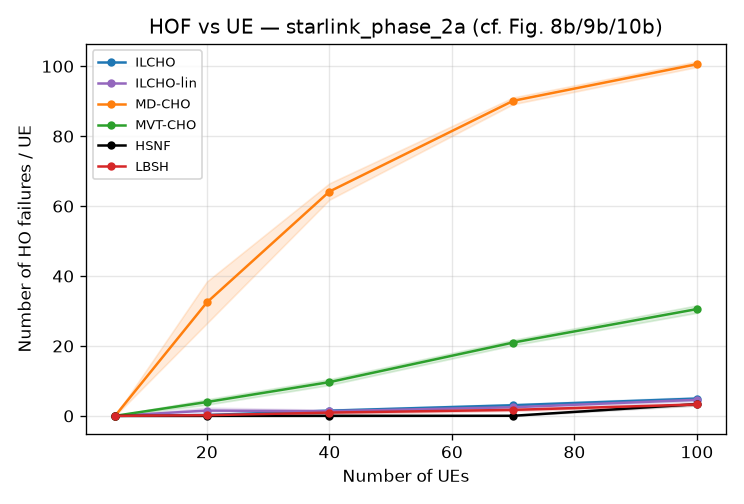
\includegraphics[width=0.85\textwidth]{images/g100_eval_starlink_phase_2a_fig_hof_vs_ue.png}
\caption{Số lần chuyển giao thất bại (HOF) theo số UE, Starlink Phase 2-a (lượt tái hiện 3).}
\label{fig:hof}
\end{figure}

\begin{figure}[H]
\centering
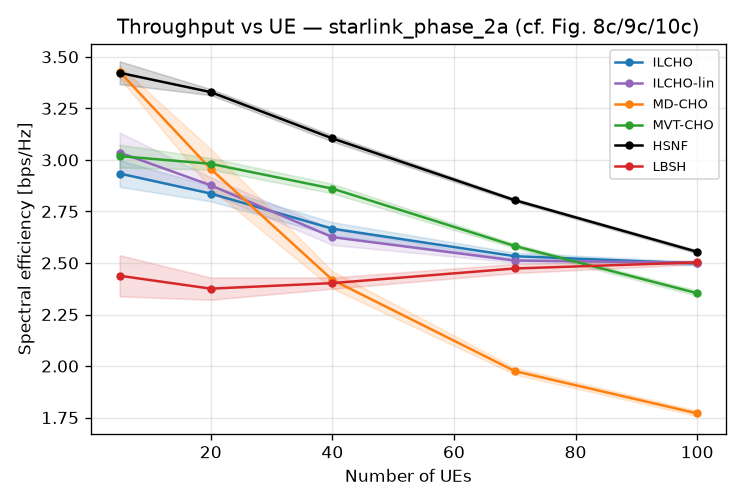
\includegraphics[width=0.85\textwidth]{images/g100_eval_starlink_phase_2a_fig_se_vs_ue.png}
\caption{Hiệu suất phổ (SE, bps/Hz) theo số UE, Starlink Phase 2-a (lượt tái hiện 3).}
\label{fig:se}
\end{figure}

\begin{figure}[H]
\centering
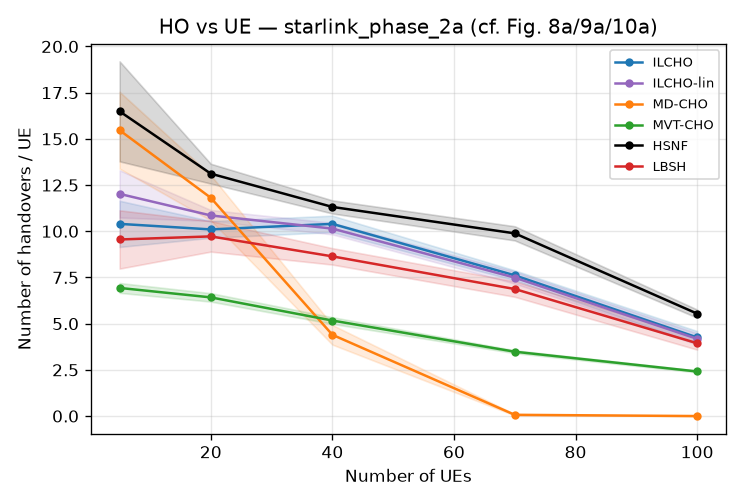
\includegraphics[width=0.85\textwidth]{images/g100_eval_starlink_phase_2a_fig_ho_vs_ue.png}
\caption{Số lần chuyển giao (HO) theo số UE, Starlink Phase 2-a (lượt tái hiện 3).}
\label{fig:ho}
\end{figure}

\begin{figure}[H]
\centering
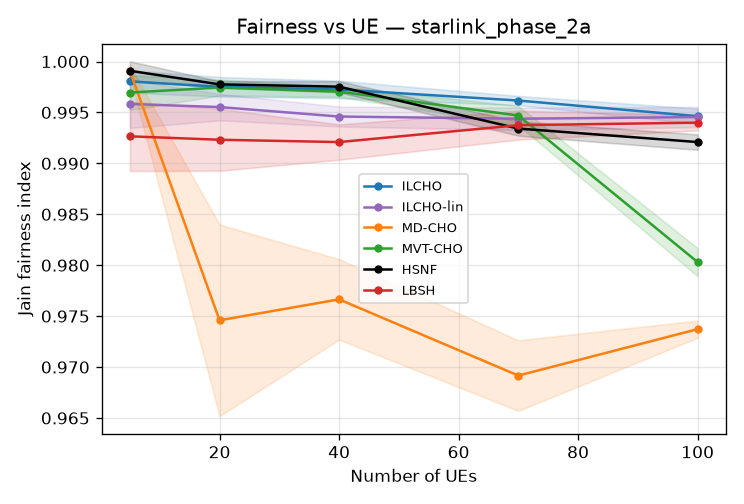
\includegraphics[width=0.85\textwidth]{images/g100_eval_starlink_phase_2a_fig_jfi_vs_ue.png}
\caption{Độ công bằng Jain (JFI) theo số UE, Starlink Phase 2-a (lượt tái hiện 3).}
\label{fig:jfi}
\end{figure}

Các kết luận đã \textbf{tái hiện được}, vững chắc qua khảo sát độ nhạy tham số:
\begin{itemize}
    \item ILCHO giữ số lần chuyển giao thất bại thấp hơn hẳn hai phương pháp truyền thống (MD-CHO, MVT-CHO) ở \textbf{mọi} mức số UE đã thử (5 đến 100) — ví dụ ở 40 UE, ILCHO thấp hơn MD-CHO khoảng 70 lần và MVT-CHO khoảng 10 lần.
    \item \textbf{Khoảng cách hiệu năng giữa ILCHO và các baseline tốt nhất (HSNF, LBSH) thu hẹp rất nhanh} khi tăng dần quy mô huấn luyện qua 3 lượt (Bảng \ref{tab:hof-rounds}), cho thấy \textbf{ngân sách huấn luyện chính là yếu tố chính} khiến các lượt tái hiện đầu chưa khớp bài báo, không phải do sai phương pháp.
    \item Số lần chuyển giao (HO) mỗi UE của ILCHO gần như ổn định khi số UE tăng (Hình \ref{fig:ho}), không tăng vọt như MD-CHO — khớp với tuyên bố "số HO ổn định" của bài báo.
    \item Độ công bằng giữa các UE (Jain's Fairness Index) đạt 0,995--0,998 trong bản tái hiện (Hình \ref{fig:jfi}) — khớp/tốt hơn con số bài báo công bố (0,9798).
    \item Hình học quỹ đạo và mô hình liên kết vô tuyến khớp sát số liệu bài báo (sai lệch vài phần trăm, xem Bảng \ref{tab:sanity}).
    \item \textbf{Kết luận trên giữ vững qua cả 3 lần huấn luyện độc lập (seed)}, không phải may rủi từ một lần chạy: ở 100 UE, khoảng cách ILCHO so với HSNF/LBSH là 1,34 lần (trung bình 3 seed), gần với 1,47 lần tính riêng từ seed đầu tiên; ba baseline không học (MD-CHO, MVT-CHO, HSNF) có độ lệch chuẩn tuyệt đối bằng 0 qua các seed — đúng như kỳ vọng, xác nhận quy trình đánh giá hoạt động chính xác.
\end{itemize}

\begin{table}[h!]
\centering
\caption{HOF trung bình mỗi UE ở 100 UE, qua 3 lượt tái hiện tăng dần quy mô.}
\label{tab:hof-rounds}
\begin{tabular}{|l|c|c|c|}
\hline
\textbf{Phương pháp} & \textbf{Lượt 1} & \textbf{Lượt 2} & \textbf{Lượt 3 (3 seed)} \\
\hline
ILCHO (đề xuất) & $\approx$47,4 & 21,1 & \textbf{4,52 $\pm$ 0,32} \\
\hline
So với baseline tốt nhất khác & -- & 6,3 lần & \textbf{1,34 lần} \\
\hline
\end{tabular}
\end{table}

Hai tuyên bố của bài báo \textbf{không tái hiện được}, đã kiểm chứng nhất quán qua cả 3 lượt (kể cả ở đúng quy mô 100 UE của lượt 3) nên đây là phát hiện thật, không phải do thiếu tài nguyên tính toán:
\begin{itemize}
    \item Bài báo cho rằng ILCHO có thông lượng cao nhất trong mọi phương pháp — trong bản tái hiện này, phương pháp \textbf{HSNF} (tham lam tối đa hoá thông lượng tức thời) luôn cao hơn ILCHO ở mọi số UE.
    \item Bài báo cho rằng hàm thưởng tuyến tính (một biến thể được thử nghiệm) huấn luyện bất ổn — trong bản tái hiện này, kể cả ở đúng quy mô 100 agent, nó hội tụ ổn định và cho chính sách gần tương đương hàm thưởng chính (sigmoid), xem Hình \ref{fig:ablation}.
\end{itemize}

\begin{figure}[H]
\centering
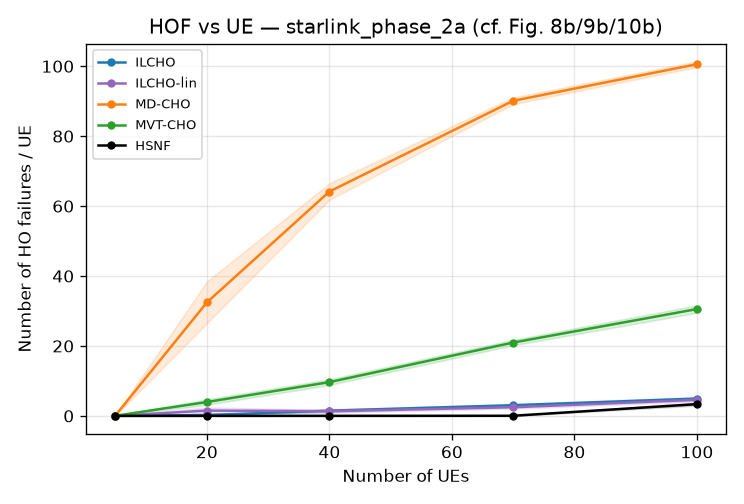
\includegraphics[width=0.85\textwidth]{images/g100_reward_ablation_fig_hof_vs_ue.png}
\caption{Thí nghiệm đối chứng hàm thưởng sigmoid so với tuyến tính (HOF theo số UE).}
\label{fig:ablation}
\end{figure}

Về mặt huấn luyện, cả ba chính sách (ILCHO-sigmoid, ILCHO-linear, LBSH) đều hội tụ mượt và đạt trạng thái bão hoà quanh episode 2.200--2.400, tức là \emph{trước khi} hết ngân sách 3.000--4.000 episode đã cấp (Hình \ref{fig:training}) — cho thấy việc huấn luyện thêm nữa (kể cả tới 30.000 episode như bài báo) khó có khả năng cải thiện đáng kể thêm ở đúng cấu hình 100 UE/600 giây này.

\begin{figure}[H]
\centering
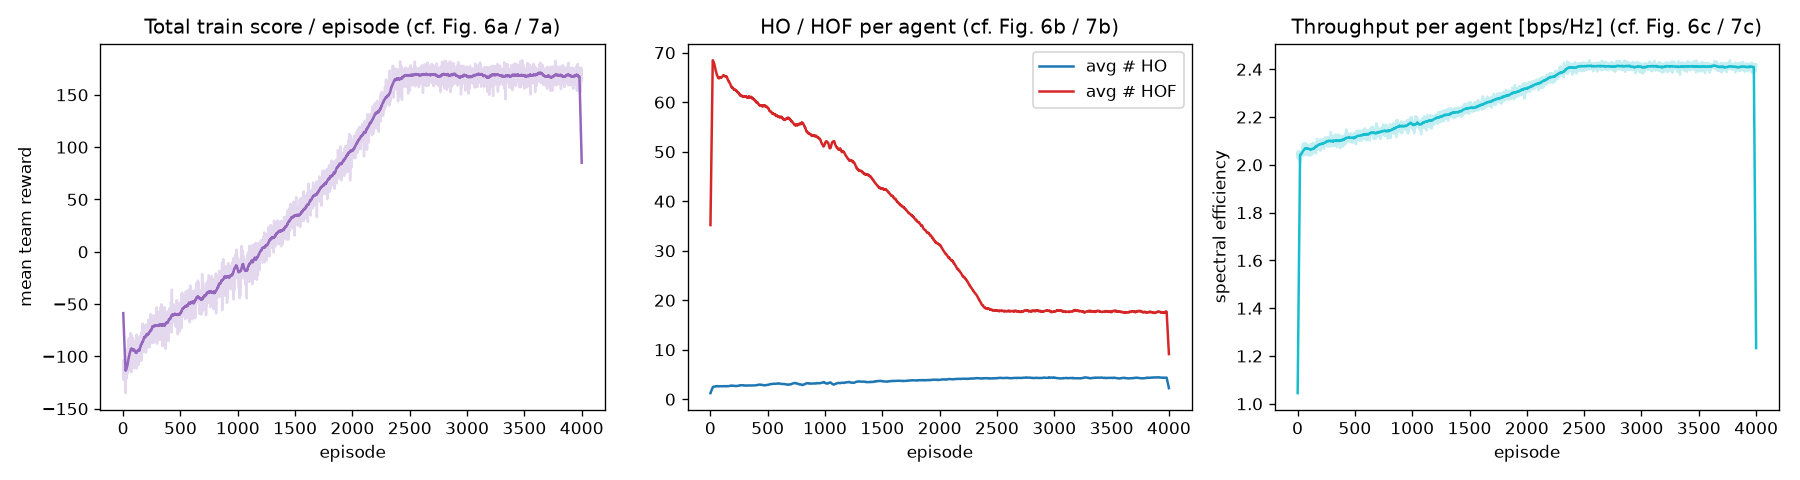
\includegraphics[width=0.85\textwidth]{images/g100_ilcho_sigmoid_training_curves.png}
\caption{Đường cong huấn luyện của chính sách ILCHO (hàm thưởng sigmoid), 100 agent, horizon 600 giây.}
\label{fig:training}
\end{figure}

\subsection{Hạn chế và những gì chưa làm được}
\begin{itemize}
    \item \textbf{Một số tham số bài báo không công bố} (tần số sóng mang chính xác, ngưỡng thực thi chuyển giao $O_{off}$, các hằng số hàm thưởng, hệ số pha chòm vệ tinh $F$, siêu tham số gốc của hai baseline HSNF/LBSH). Em đã tự chọn giá trị hợp lý và kiểm chứng độ nhạy với ba trong năm tham số này (kết luận về thứ hạng các phương pháp không đổi dù giá trị tham số thay đổi) — hai tham số còn lại (hằng số hàm thưởng, siêu tham số gốc của baseline) chưa kiểm chứng được đầy đủ. Đây là giới hạn \textbf{không thể tự đóng được} nếu không liên hệ trực tiếp nhóm tác giả bài báo.
    \item Hai phương pháp so sánh (HSNF, LBSH) đang dùng \textbf{bản triển khai rút gọn} của em, chưa cài đúng theo hai bài báo tham chiếu gốc mà ILCHO trích dẫn — đây là việc còn có thể làm thêm nếu có thời gian, và nhiều khả năng là nguyên nhân của hai điểm không tái hiện được ở trên.
    \item Do giới hạn bộ nhớ GPU hiện có (8 GB VRAM), kích thước lô dữ liệu (batch size) khi huấn luyện là 8, chưa đúng hoàn toàn với giá trị 32 mà bài báo công bố.
    \item Mới kiểm chứng độ ổn định qua 3 lần huấn luyện độc lập (khuyến nghị thống kê tối thiểu); có thể tăng lên 5 lần nếu muốn kết quả chặt hơn.
    \item Các kết quả ở chòm vệ tinh Phase 1-a và kịch bản hybrid đều là \textbf{chuyển giao chính sách không huấn luyện lại} (zero-shot) từ chính sách đã huấn luyện trên Phase 2-a, chưa huấn luyện riêng cho từng chòm vệ tinh.
\end{itemize}

\subsection{Kế hoạch tiếp theo}
\begin{enumerate}
    \item Đọc và cài đặt lại đúng hai phương pháp so sánh (HSNF, LBSH) theo đúng hai bài báo tham chiếu gốc — đây là việc có khả năng làm rõ nhất liệu hai kết luận chưa tái hiện được ở trên là do bản triển khai rút gọn hay là khác biệt thật.
    \item Cân nhắc liên hệ nhóm tác giả bài báo để xin các tham số chưa công bố.
    \item Nếu còn thời gian: huấn luyện riêng cho từng chòm vệ tinh (hiện đang dùng chuyển giao chính sách từ chòm vệ tinh chính sang các chòm khác), và tăng số lần huấn luyện độc lập lên 5 seed để có khoảng tin cậy chặt hơn.
\end{enumerate}

\newpage
\section*{KẾT LUẬN CHUNG}
\addcontentsline{toc}{section}{\numberline{}KẾT LUẬN CHUNG}
Qua đồ án này, em đã khảo sát chi tiết bài báo ILCHO — một cách tiếp cận có cơ sở kỹ thuật vững cho bài toán chọn vệ tinh đích trong chuyển giao NTN, với đóng góp cốt lõi là thiết kế không gian hành động giúp học tăng cường đa tác tử mở rộng được tới quy mô mega-constellation, điều mà các công trình MARL trước đó chưa làm được. Hạn chế lớn nhất về mặt học thuật của bài báo là cách dùng từ "dự đoán" không chính xác (bài toán thực chất là ra quyết định trên thông tin tất định), còn về mặt thực nghiệm là thiếu nhiều chi tiết cần thiết để tái lập đầy đủ kết quả.

Sau ba lượt tái hiện tăng dần quy mô, tuyên bố cốt lõi của bài báo — một cơ chế chuyển giao có điều kiện, điều khiển bằng học tăng cường đa tác tử, giữ số chuyển giao thất bại thấp và ổn định trong chòm vệ tinh mật độ cao, nơi các phương pháp truyền thống thất bại khi tải tăng — \textbf{đã được tái hiện rõ ràng và vững chắc}, và được kiểm chứng thêm qua nhiều lần huấn luyện độc lập. Khoảng cách với bài báo ở vùng tải cao nhất đã thu hẹp mạnh nhờ huấn luyện đúng quy mô bài báo công bố. Một số chi tiết (thông lượng cao nhất; độ ổn định của biến thể hàm thưởng tuyến tính) chưa tái hiện được và đã được em báo cáo trung thực như các phát hiện riêng, không che giấu.

\noindent\emph{Toàn bộ mã nguồn, số liệu chi tiết và các báo cáo kỹ thuật đầy đủ được lưu tại kho mã nguồn của đề tài.}

\newpage
\phantomsection\addcontentsline{toc}{section}{\numberline {}TÀI LIỆU THAM KHẢO}
\bibliographystyle{IEEEtran}
\bibliography{TaiLieuThamKhao_ILCHO}
\newpage
\end{document}
